
\documentclass[addpoints]{exam}
% Used to insert images
\usepackage[utf8]{inputenc}
\usepackage{siunitx}
\usepackage{graphicx}
\usepackage{color}
\usepackage{tikz}
\usetikzlibrary{shapes.geometric, positioning, arrows.meta}
\usepackage{amsmath} 

\printanswers

\newcommand{\event}{Modern Physics}
\def\type{0}

\setlength\fillinlinelength{\textwidth}
\CorrectChoiceEmphasis{\color{red}\bfseries}
\SolutionEmphasis{\color{red}\bfseries}

\setlength\answerclearance{2pt}
\pagestyle{headandfoot}
% Adds a line to the top of the page
\runningheadrule
% The three braces correspond to the different parts of the header: the left is the top left text, middle is top middle, and right is top right.
\runningheader{\event}{\tournament}{\ifnum\type=1 Class Set Test \else Full Name:\hspace{1cm} \fi }
% Adds a line to the bottom of the page
\runningfootrule
% The three braces correspond to the different parts of the footer: the left is the bottom left text, middle is bottom middle, and right is bottom right.
% Doesn't include the title page in the page count 
% \runningfooter{}{Page \the\numexpr\thepage-1\   of \the\numexpr\numpages-1}{}
% Uncomment the line below if you want to include the title page in the page count 
\runningfooter{}{Page \thepage\   of \numpages}{}

\begin{document}
\begin{center}
    {\huge Grade 12 Physics \\ \event
    % Writes key if the answers are shown, otherwise writes test
    \ifprintanswers 
     \space Key
    \else 
     \space \ifnum\type<2 Test \fi \ifnum\type=1 \textbf{(CLASS SET)} \fi \ifnum\type=2 Answer Sheet \fi
    \fi \\ \vspace{3mm}\tournament\vspace{1mm}}
\end{center}
% Change to any picture or just some \vspace{.3\textheight} to leave it blank. [h] ensures that the image is placed in the same place in the document as in the code
\begin{figure}[h]
    \centering
    \includegraphics[height=.3\textheight, width=.6\textwidth, keepaspectratio]{}
\begin{figure}
    \centering
    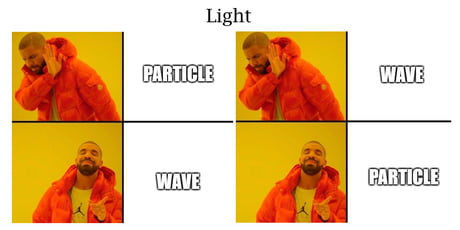
\includegraphics[width=0.5\linewidth]{particle-duality-meme-drake.jpg}
    \label{fig:enter-label}
\end{figure}
\end{figure}


\begin{center}
    First Name: \ifprintanswers
    \underline{\hspace{3.5cm}}\textbf{KEY}\underline{\hspace{5.5cm}}\\\vspace{5mm}
    \else
        \underline{\hspace{10cm}}\\ \vspace{5mm}
    \fi
    Last Name: \underline{\hspace{10cm}}\\ \vspace{5mm}

\end{center}

% Change the list below to reflect the instructions for your test
\noindent\textbf{\underline{Directions:}}
\begin{itemize}
    % If the test is a class set, an instruction will appear to not write on the test paper.
    \ifnum\type=1 \item \textbf{This test is a class set.} Please do not write any answers on this paper. \fi
    % Adds an instruction 
    \item Please answer to 2 decimal points
    \item The test is designed to be completed in 75 minutes
\end{itemize}
\begin{center}
\textit{For grading use only}\\
% The gradetable has a number of rows that automatically updates. This is not very accurate because of the variance in question size, but it can serve as a starting point. You will probably need to manually update the number of rows of the gradetable (change '\the\numexpr\numpages/13+1' to the desired number of rows).
\multirowgradetable{1}[pages]   
\end{center}

\newpage

\begin{questions}


\section*{Multiple Choice (10 marks)}
\vspace{5mm}

\question[1] Which phenomenon directly demonstrates the particle nature of light?
\begin{choices}
    \correctchoice Photoelectric effect
    \choice Diffraction
    \choice Interference
    \choice Polarization
\end{choices}

\question[1] In special relativity, proper time is measured by:
\begin{choices}
    \correctchoice A clock at rest relative to the event
    \choice A clock moving at constant velocity
    \choice Any inertial observer
    \choice An accelerating observer
\end{choices}

\question[1] Millikan's oil drop experiment determined:
\begin{choices}
    \choice Electron mass
    \correctchoice Elementary charge
    \choice Planck's constant
    \choice Speed of light
\end{choices}

\question[1] The Lorentz factor γ for v = 0.8c is:
\begin{choices}
    \choice 1.25
    \choice 2.00
    \correctchoice 1.67
    \choice 0.60
\end{choices}

\question[1] Which best describes wave-particle duality?
\begin{choices}
    \choice Particles behave as waves at high speeds
    \choice Waves can become particles in electric fields
    \choice Photons switch between wave and particle states
    \correctchoice All matter has both wave and particle properties
\end{choices}

\question[1] The work function of a metal is 2.3 eV. The minimum light frequency needed for photoemission is:
\begin{choices}
    \choice $3.5 \times 10^{14}$ Hz
    \choice $1.1 \times 10^{15}$ Hz
    \choice $2.3 \times 10^{15}$ Hz
    \correctchoice $5.6 \times 10^{14}$ Hz
\end{choices}

\question[1] A meter stick moving at 0.6c appears contracted to:
\begin{choices}
    \choice 0.60 m
    \choice 1.00 m
    \correctchoice 0.80 m
    \choice 1.25 m
\end{choices}

\question[1] The ultraviolet catastrophe refers to:
\begin{choices}
    \choice X-ray production in cathode tubes
    \correctchoice Classical theory's failure at short wavelengths
    \choice Quantum tunneling effects
    \choice Relativistic length contraction
\end{choices}

\question[1] Which is NOT a consequence of special relativity?
\begin{choices}
    \choice Time dilation
    \choice Length contraction
    \correctchoice Mass variation with speed
    \choice Simultaneity relativity
\end{choices}

\question[1] The rest energy of a proton ($m = 1.67 \times 10^{-27}$ kg) is:
\begin{choices}
    \choice $1.50 \times 10^{-10}$ J
    \correctchoice $1.50 \times 10^{-10}$ J
    \choice $2.25 \times 10^{-19}$ J
    \choice $4.50 \times 10^{-19}$ J
\end{choices}

\section*{Long Answer (40 marks)}

\question Relativistic Space Travel
\begin{parts}
    \part[4] A spaceship travels to Alpha Centauri (4.37 ly away) at 0.95c. Calculate the travel time experienced by astronauts.
    \part[4] Determine the distance to Alpha Centauri in the spaceship's frame.
\end{parts}
\begin{solution}
    \textbf{11. Relativistic Space Travel}  

\textbf{(a) Travel time experienced by astronauts:}  

The time experienced by astronauts (proper time) is given by time dilation:  
\[
\Delta t' = \Delta t \sqrt{1 - \frac{v^2}{c^2}}
\]
where  
\[
\Delta t = \frac{d}{v} = \frac{4.37 \text{ ly}}{0.95c} = 4.60 \text{ years}
\]
Thus,  
\[
\Delta t' = 4.60 \times \sqrt{1 - (0.95)^2}
\]
\[
= 4.60 \times \sqrt{1 - 0.9025}
\]
\[
= 4.60 \times \sqrt{0.0975}
\]
\[
= 4.60 \times 0.3123 = 1.44 \text{ years}
\]

\textbf{(b) Distance to Alpha Centauri in the spaceship’s frame:}  

Length contraction is given by:  
\[
L' = L \sqrt{1 - \frac{v^2}{c^2}}
\]
Substituting values:  
\[
L' = 4.37 \times \sqrt{0.0975}
\]
\[
= 4.37 \times 0.3123
\]
\[
= 1.37 \text{ ly}
\]
\end{solution}


\question Photoelectric Analysis
\begin{parts}
    \part[4] Light with λ = 250 nm strikes a metal (work function 4.7 eV). Calculate the maximum kinetic energy of emitted electrons.
    \part[4] If intensity doubles, what happens to: (i) Stopping potential (ii) Photocurrent?
\end{parts}
\begin{solution}
\textbf{12. Photoelectric Analysis}  

\textbf{(a) Maximum kinetic energy of emitted electrons:}  

The energy of the incident photon is given by:  
\[
E = \frac{hc}{\lambda}
\]
Using \( h = 6.63 \times 10^{-34} \) J·s and \( c = 3.00 \times 10^8 \) m/s,  
\[
E = \frac{(6.63 \times 10^{-34}) (3.00 \times 10^8)}{250 \times 10^{-9}}
\]
\[
= \frac{1.989 \times 10^{-25}}{250 \times 10^{-9}}
\]
\[
= 7.96 \times 10^{-19} \text{ J}
\]
Convert to eV (1 eV = \(1.602 \times 10^{-19}\) J):  
\[
E = \frac{7.96 \times 10^{-19}}{1.602 \times 10^{-19}} = 4.97 \text{ eV}
\]
The maximum kinetic energy of the emitted electrons is given by:  
\[
KE_{\max} = E - \phi
\]
\[
KE_{\max} = 4.97 - 4.7 = 0.27 \text{ eV}
\]

\textbf{(b) Effect of doubling intensity:}  

(i) \textbf{Stopping potential:}  
The stopping potential \( V_s \) is given by:  
\[
eV_s = KE_{\max}
\]
Since \( KE_{\max} \) depends only on photon energy (not intensity), \( V_s \) remains unchanged.  

(ii) \textbf{Photocurrent:}  
Increasing intensity increases the number of incident photons per second, leading to a higher emission rate of electrons. Thus, photocurrent increases.  

\end{solution}

\vspace{1cm}

\question Charge Quantization
\begin{parts}
    \part[4] In Millikan's experiment, an oil drop with 8 excess electrons is suspended when E = \SI{2.1e4}{N/C}. Find the drop's mass.
    \part[4] Calculate possible charges for a drop experiencing forces of \SI{3.2e-14}{N} in the same field.
\end{parts}
\begin{solution}

\textbf{(a) Finding the mass of the oil drop:}  

The force on the oil drop due to the electric field is balanced by its weight:  
\[
F_e = F_g
\]
\[
qE = mg
\]
The charge on the drop is given by:  
\[
q = n e = 8 \times (1.602 \times 10^{-19}) = 1.2816 \times 10^{-18} \text{ C}
\]
Solving for mass:  
\[
m = \frac{qE}{g}
\]
Substituting values:  
\[
m = \frac{(1.2816 \times 10^{-18}) (2.1 \times 10^4)}{9.81}
\]
\[
= \frac{2.69136 \times 10^{-14}}{9.81}
\]
\[
= 2.74 \times 10^{-15} \text{ kg}
\]

\textbf{(b) Possible charges for a drop experiencing a force of \( 3.2 \times 10^{-14} \) N:}  

Since the force due to the electric field is given by:  
\[
F_e = qE
\]
Solving for \( q \):  
\[
q = \frac{F_e}{E}
\]
\[
= \frac{3.2 \times 10^{-14}}{2.1 \times 10^4}
\]
\[
= 1.52 \times 10^{-18} \text{ C}
\]
Since charge is quantized in units of \( e = 1.602 \times 10^{-19} \), the possible values are:  
\[
q = n e
\]
\[
n = \frac{1.52 \times 10^{-18}}{1.602 \times 10^{-19}} \approx 9.5
\]
Since \( n \) must be an integer, the closest possible values are for \( n = 9 \) or \( n = 10 \), meaning:  
\[
q = 9(1.602 \times 10^{-19}) = 1.44 \times 10^{-18} \text{ C}
\]
\[
q = 10(1.602 \times 10^{-19}) = 1.60 \times 10^{-18} \text{ C}
\]
\end{solution}


\question[8] Particle-Wave Duality
\begin{parts}
    \part[4] Calculate de Broglie wavelength for a 150 g baseball moving at 40 m/s.
    \part[4] Why don't we observe wave properties for macroscopic objects?
\end{parts}
\begin{solution}
\textbf{(a) de Broglie wavelength of a baseball:}  

The de Broglie wavelength is given by:  
\[
\lambda = \frac{h}{mv}
\]
Substituting values (\( h = 6.63 \times 10^{-34} \) J·s, \( m = 0.150 \) kg, \( v = 40 \) m/s):  
\[
\lambda = \frac{6.63 \times 10^{-34}}{(0.150)(40)}
\]
\[
= \frac{6.63 \times 10^{-34}}{6.00}
\]
\[
= 1.10 \times 10^{-34} \text{ m}
\]

\textbf{(b) Why don’t we observe wave properties for macroscopic objects?}  

Wave-like properties such as diffraction and interference are only noticeable when the wavelength is comparable to or larger than the object's size or the experimental setup's dimensions.  

For macroscopic objects, the de Broglie wavelength is extremely small (as seen in part (a)), making wave effects undetectable. In contrast, for electrons and other small particles, the wavelength is significant enough to observe diffraction and interference patterns.  

\end{solution}


\question[8] Blackbody Radiation
\begin{parts}
    \part[4] A star emits peak radiation at 400 nm. Estimate its surface temperature.
    \part[4] If the star's radius is \SI{7e8}{m}, calculate its total power output.
\end{parts}
\begin{solution}
\textbf{(a) Estimating the star’s surface temperature:}  

We use Wien’s displacement law:  
\[
\lambda_{\text{max}} T = 2.898 \times 10^{-3} \text{ m·K}
\]
Given \( \lambda_{\text{max}} = 400 \) nm = \( 400 \times 10^{-9} \) m, solving for \( T \):  
\[
T = \frac{2.898 \times 10^{-3}}{400 \times 10^{-9}}
\]
\[
= \frac{2.898 \times 10^{-3}}{4.00 \times 10^{-7}}
\]
\[
= 7.25 \times 10^3 \text{ K} = 7250 \text{ K}
\]

\textbf{(b) Calculating the total power output:}  

The total power output of a star is given by the Stefan-Boltzmann law:  
\[
P = \sigma A T^4
\]
where  
\( \sigma = 5.670 \times 10^{-8} \) W/m\(^2\)K\(^4\),  
\( R = 7.00 \times 10^8 \) m,  
\( A = 4\pi R^2 \),  
\( T = 7250 \) K.  

First, calculate the surface area:  
\[
A = 4 \pi (7.00 \times 10^8)^2
\]
\[
= 4 \pi (4.90 \times 10^{17})
\]
\[
= 6.16 \times 10^{18} \text{ m}^2
\]

Now, calculate the power:  
\[
P = (5.670 \times 10^{-8}) (6.16 \times 10^{18}) (7250)^4
\]
\[
= (5.670 \times 10^{-8}) (6.16 \times 10^{18}) (2.76 \times 10^{15})
\]
\[
= (5.670 \times 10^{-8}) (1.70 \times 10^{34})
\]
\[
= 9.64 \times 10^{26} \text{ W}
\]

Thus, the total power output of the star is approximately  
\[
P \approx 9.64 \times 10^{26} \text{ W}
\]
\end{solution}


\end{questions}

\end{document}
